\documentclass{article}
\usepackage[paperwidth=14in,paperheight=6.2in,margin=0.25in]{geometry}
\usepackage{tikz}
\renewcommand{\familydefault}{\sfdefault}
\usetikzlibrary{arrows.meta, positioning, calc, backgrounds}

\definecolor{darknavy}{HTML}{1B263B}
\definecolor{cardioblue}{HTML}{E8F0FE}
\definecolor{cardiogreen}{HTML}{E6F4EA}
\definecolor{cardioorange}{HTML}{FEF7E0}
\definecolor{cardiopurple}{HTML}{F3E8FD}
\definecolor{borderblue}{HTML}{1A73E8}
\definecolor{bordergreen}{HTML}{137333}
\definecolor{borderorange}{HTML}{E37400}
\definecolor{borderpurple}{HTML}{9334E6}
\definecolor{accentred}{HTML}{C5221F}
\definecolor{bannerbg}{HTML}{F8F9FA}
\definecolor{bannerborder}{HTML}{BDC1C6}

\pagestyle{empty}
\begin{document}
\begin{center}
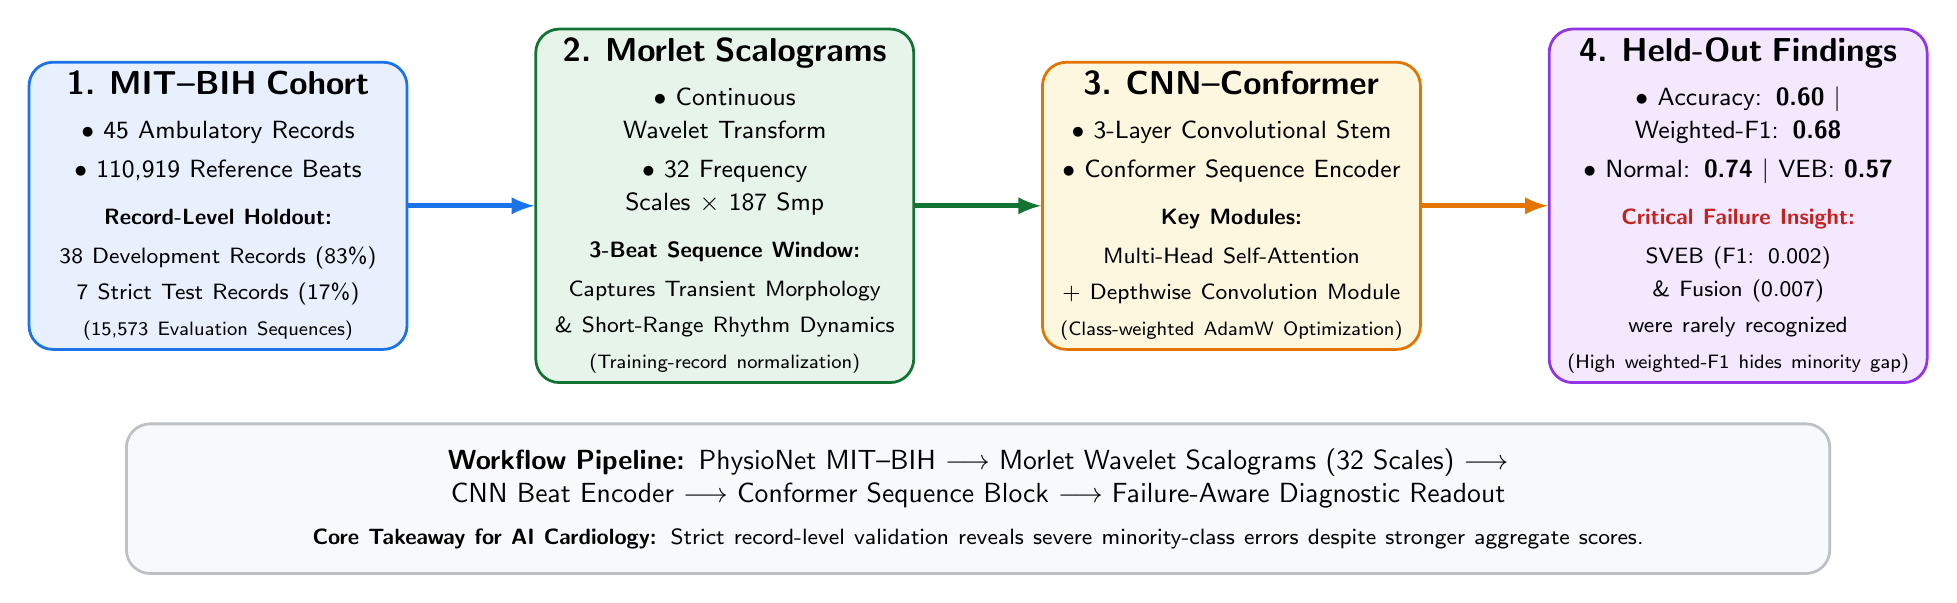
\begin{tikzpicture}[font=\sffamily, >=latex]
  % Stage Box Styles
  \tikzstyle{stagebox} = [draw=darknavy, rounded corners=3mm, minimum width=4.8cm,
    minimum height=3.6cm, align=center, line width=1pt]

  % Stage 1: Cohort & Data
  \node[stagebox, fill=cardioblue, draw=borderblue, text width=4.5cm] (data) at (0, 0)
    {{\textbf{\large 1. MIT--BIH Cohort}}\\[4pt]
     {\small $\bullet$ 45 Ambulatory Records}\\[2pt]
     {\small $\bullet$ 110{,}919 Reference Beats}\\[5pt]
     \textbf{\footnotesize Record-Level Holdout:}\\[2pt]
     {\footnotesize 38 Development Records (83\%)}\\[1pt]
     {\footnotesize 7 Strict Test Records (17\%)}\\[1pt]
     {\scriptsize (15{,}573 Evaluation Sequences)}};

  % Stage 2: Representation & CWT
  \node[stagebox, fill=cardiogreen, draw=bordergreen, text width=4.5cm, right=1.6cm of data] (prep)
    {{\textbf{\large 2. Morlet Scalograms}}\\[4pt]
     {\small $\bullet$ Continuous Wavelet Transform}\\[2pt]
     {\small $\bullet$ 32 Frequency Scales $\times$ 187 Smp}\\[5pt]
     \textbf{\footnotesize 3-Beat Sequence Window:}\\[2pt]
     {\footnotesize Captures Transient Morphology}\\[1pt]
     {\footnotesize \& Short-Range Rhythm Dynamics}\\[1pt]
     {\scriptsize (Training-record normalization)}};

  % Stage 3: Architecture
  \node[stagebox, fill=cardioorange, draw=borderorange, text width=4.5cm, right=1.6cm of prep] (model)
    {{\textbf{\large 3. CNN--Conformer}}\\[4pt]
     {\small $\bullet$ 3-Layer Convolutional Stem}\\[2pt]
     {\small $\bullet$ Conformer Sequence Encoder}\\[5pt]
     \textbf{\footnotesize Key Modules:}\\[2pt]
     {\footnotesize Multi-Head Self-Attention}\\[1pt]
     {\footnotesize $+$ Depthwise Convolution Module}\\[1pt]
     {\scriptsize (Class-weighted AdamW Optimization)}};

  % Stage 4: Findings
  \node[stagebox, fill=cardiopurple, draw=borderpurple, text width=4.5cm, right=1.6cm of model] (output)
    {{\textbf{\large 4. Held-Out Findings}}\\[4pt]
     {\small $\bullet$ Accuracy: \textbf{0.60} $\mid$ Weighted-F1: \textbf{0.68}}\\[2pt]
     {\small $\bullet$ Normal: \textbf{0.74} $\mid$ VEB: \textbf{0.57}}\\[5pt]
     {\color{accentred}\textbf{\footnotesize Critical Failure Insight:}}\\[2pt]
     {\footnotesize SVEB (F1: 0.002) \& Fusion (0.007)}\\[1pt]
     {\footnotesize were rarely recognized}\\[1pt]
     {\scriptsize (High weighted-F1 hides minority gap)}};

  % Connecting Arrows with Colors
  \draw[->, line width=1.8pt, color=borderblue] (data.east) -- (prep.west);
  \draw[->, line width=1.8pt, color=bordergreen] (prep.east) -- (model.west);
  \draw[->, line width=1.8pt, color=borderorange] (model.east) -- (output.west);

  % Bottom Enclosed Summary Banner (Zero text overlap)
  \node[draw=bannerborder, fill=bannerbg, rounded corners=3mm, line width=1pt,
        text width=21cm, align=center, inner sep=9pt, anchor=north] (banner) at ($(prep.south)!0.5!(model.south) + (0, -0.7cm)$)
    {{\textbf{\normalsize Workflow Pipeline:}} PhysioNet MIT--BIH $\longrightarrow$ Morlet Wavelet Scalograms (32 Scales) $\longrightarrow$ CNN Beat Encoder $\longrightarrow$ Conformer Sequence Block $\longrightarrow$ Failure-Aware Diagnostic Readout\\[3pt]
     {\footnotesize \textbf{Core Takeaway for AI Cardiology:} Strict record-level validation reveals severe minority-class errors despite stronger aggregate scores.}};

\end{tikzpicture}
\end{center}
\end{document}
